\documentclass[a4paper]{article}
\usepackage[T1]{fontenc}
\usepackage[utf8]{inputenc}
\usepackage{lmodern}
\usepackage{graphicx}
\usepackage{hyperref}
%\usepackage{tipa}

\usepackage{setspace} 
\DeclareUnicodeCharacter{00A0}{ }

\begin{document}
\begin{titlepage}

\newcommand{\HRule}{\rule{\linewidth}{0.7mm}} % Defines a new command for the horizontal lines, change thickness here


\center % Center everything on the page
 
%----------------------------------------------------------------------------------------
%	HEADING SECTIONS
%----------------------------------------------------------------------------------------

\textsc{\LARGE University of Tromsø}\\[1.5cm] % Name of your university/college
\textsc{\Large INF-2900}\\[0.5cm] % Major heading such as course name
\textsc{\large Software Engineering}\\[0.5cm] % Minor heading such as course title

%----------------------------------------------------------------------------------------
%	TITLE SECTION
%----------------------------------------------------------------------------------------

\HRule \\[0.5cm]
{ \huge \bfseries Turi}\\[0.5cm] % Title of your document
\HRule \\[3cm]
 
%----------------------------------------------------------------------------------------
%	AUTHOR SECTION
%----------------------------------------------------------------------------------------

% If you don't want a supervisor, uncomment the two lines below and remove the section above
\Large \emph{Group:}\\
1\\[2cm] % Your name
% title
%----------------------------------------------------------------------------------------
%	DATE SECTION
%----------------------------------------------------------------------------------------

\textsc{\large Spring 2015}\\[4cm] % Date, change the \today to a set date if you want to be precise

%----------------------------------------------------------------------------------------
%	LOGO SECTION
%----------------------------------------------------------------------------------------


\includegraphics{pictures/UiT_samarbeidslogo_bokmal_300ppi.png}\\[1cm] 
% Include a department/university logo - this will require the graphicx package
 
%----------------------------------------------------------------------------------------

\vfill % Fill the rest of the page with whitespace

\end{titlepage}
% END TITLE PAGE %

\tableofcontents
\pagebreak


\section{Introduction}
Imagine you want to go on a trip - to Norway for example. You ask you friends to join you but they reject because they can not afford the money or they have no spare time. What now? You can either go alone or try to find some people who can join you. The first place we look today is on the world wide web. We already can find some portals where you can find partners for your trip. But what about planning your actually trip? We couldn’t find a tool which allows you to plan your trip in detail. Planning your trip gets especially difficult if you find your trip mates online and you can not meet because you live too far away from each other. You can now either use the phone or create e.g. some Facebook group. Still those ways lack of several features we want to implement in our trip planner which makes it unique. In fact we came up with the idea to create a a trip planner which offers a combination between socialising and planning for your trips.

\subsection{The product name: turi}
The name derived from the Norwegian word “tur” (a trip/a walk). turi was short and pregnant enough and sounds best to the ear. It is also a Norwegian name, but this will be no problem when we think about topics like a trademark etc.

\subsection{Summary of goals (planned functionalities)}
The following functionalities should be supported (bold means that we they were implemented during the course sprints):
\begin{itemize}
  \item {\textbf{Discuss with participants}}
  \item {\textbf{Event management (for appointments top plan)}}
  \item {\textbf{Route planning}}
  \item {\textbf{Equipment planning}}
  \item {\textbf{Gallery to visualize your trip experiences}}
  \item {\textbf{Blog about your experience}}
  \item {\textbf{Share your trip (public/private)}}
  \item {Copy a previous trip from others (e.g. routes)}
  \item {Rating functionality and other common social functions (commenting, likes..)
  \begin{itemize}
    \item {Friend requests}
  \end{itemize}}
  \item {\textbf{Explore trips based on their location}}
  \item {Badges and rewards for participating and using Turi}
  \item {Search and find trips according your interests}
\end{itemize}

\noindent
Finally we were not able to implement all of our goals and we had tons of more ideas. But for the first release of turi (1.0.0) we decided to require all these features above.


\section{The development process}
\subsection{Git}
We use github.com instead of the git repository supplied to us from the school, this gave us the opportunity to work outside the school network. In addition it gave us the ability to use 3rd party applications, this is explained the following subsections. The githib repository address is: https://github.com/turi-inc/turi.

\subsubsection{Travis CI}
Travis CI is a hosted continuous integration service. It is integrated with GitHub and provides testing for our project. So when we created a pull request on the development branch of the Github repository, Travis would test our new code automatically and give us a clear indication if the test was passing or not. When the pull request is merged with the development branch it would be tested once again by Travis to be sure that everything was working correctly before the pull request is automatically merged with the master branch of the repository. The log from Travis is public and can be seen here: https://travis-ci.org/turi-inc/turi/builds.

\begin{figure}
  \begin{center}
    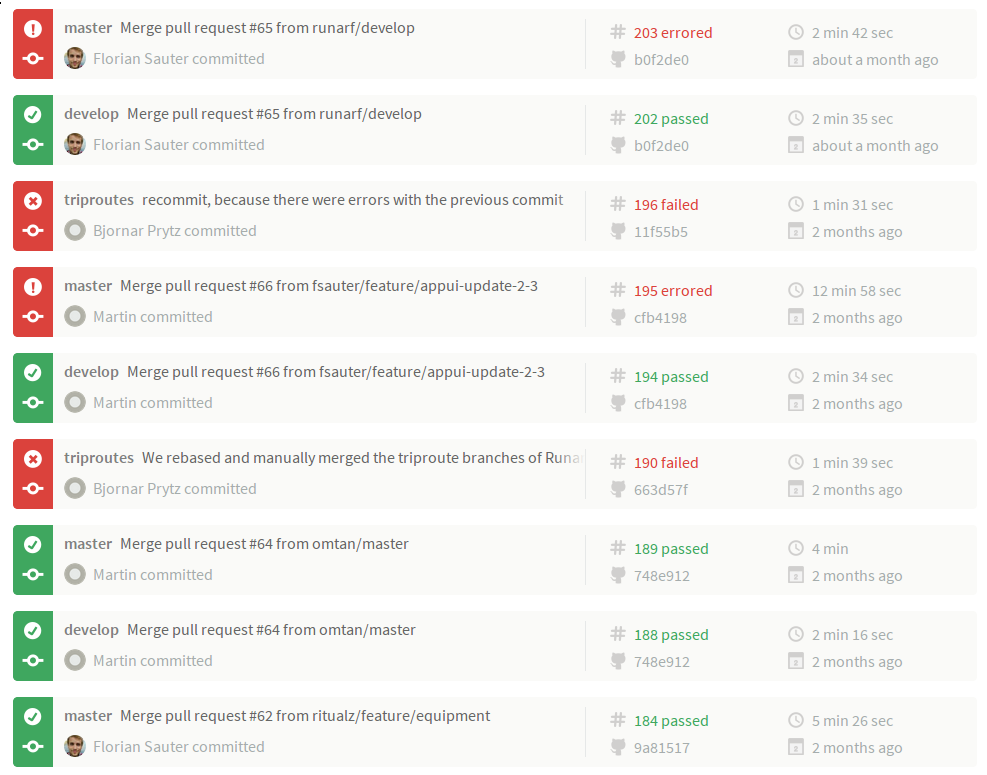
\includegraphics[scale=0.45]{pictures/Travis_buildlog.png}
    \caption{A sample of the build logs from Travis CI}
    \label{fig:}
  \end{center}
\end{figure}


\subsubsection{Heroku}
Heroku is a cloud platform which host our project for free. When a pull request is merged with the master branch it's automatically pushed to Heroku. This gives us and other people to see a preview of the project. We had some minor problem getting this to work properly since we use Sqlite3 when we develop, but Heroku does not support this and so we had to switch over to postgres in the production environment.

\subsubsection{CodeClimate}
Is also a 3rd party application which checks our code for test coverage, complexity and duplications. The check is done on the master branch of the repository, every time a new pull request is merged with the branch. It gives us an indication about the code health and grades our code, on the basis of test coverage, complexity and duplications. The summary of the code climate of out project can be found here: https://codeclimate.com/github/turi-inc/turi. \\
CodeClimate also have some cool features like Trends over the "health" of our code over time, and the location "hotspots" in the code.  

\begin{figure}
  \begin{center}
    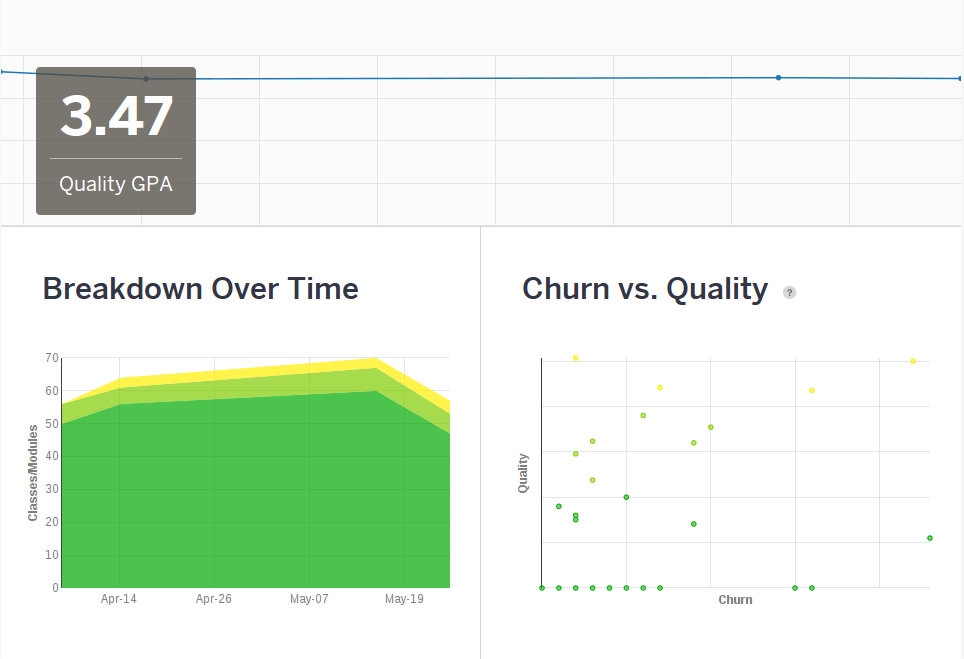
\includegraphics[scale=0.45]{pictures/trends_code.png}
    \caption{CodeClimate trends}
    \label{fig:}
  \end{center}
\end{figure}

\subsubsection{Hakiri}
This 3rd party application is used to show if there is any gem which is not up to date, and if there is any known security claws in any of the gems we use in our project.

\section{Design of the site}

\section{Gems}
We use several gems in our project, this means that we not need find up the wheel for already created features, and we can focus on our own feature. All the gems used can be found in the gemfile in the project source, but the most important ones are:
\subsection{Devise}
Devise is a popular authentication solution for Rails based on Warden \cite{devise}. \\
In the first iterations we created our own authentication system, but we found out that we could use \textit{Devise}, after the lecture about authentication. This made it possible to focus on other task in the project, and not focus on making a secure and safe authentication system. 

\subsection{Pundit}
\textit{Pundit} is an authorization system, which we use in almost all features in projects, 

\subsection{Leaflet}
\textit{Leaflet}\cite{leaflet} is a JavaScript library that let us implement the interactive map for the routes. Before discovering \textit{Leaflet}, we looked at a similar gem from Google, but it was too heavy for our requirements. As an example, Google Maps seemed to snap waypoints to the nearest road, which is counter-productive for us since we want the users to be able to plan any kind of trip, including hikes.


\subsection{rails-asserts}

\subsection{Geocoder}
\textit{Geocoder} is a so called "complete geocoding solution for Ruby"\cite{geocoder}, it provides a location based on IP, location and so on, in the project we use it for location based search, for example in the trip start and end location. 

\subsection{Puma}
\textit{Puma} is a "simple, fast, threaded, and highly concurrent HTTP 1.1 server for Ruby/Rack applications."\cite{puma}. Heroku recommend \textit{Puma} over the stock rails server (WEBrick) by saying that: "While WEBrick should be fine for development, it was not designed to handle a high concurrent workload that a Ruby app must serve in production. A production web server should be used instead."\cite{heroku_webserver}. Even tho Heroku only uses one core (for the free program), this secures that the project is ready for a deployment onto a multi-core server in the future.  


\section{Trip Features}
The trip and it's features are the main focus of our project. 
\subsection{Discuss}
\subsection{Event management}
\subsection{Equipment planning}
\subsection{Gallery}
\subsection{Blog}
The blog platform allows a trip editor to create a blog associated with the trip. The user can edit the blog through a simple editor interface which also allows for urls and images. A blog can be marked as public, which means that non-participants can read it. The platform has a blog index list which lists the blogs in order of creation and shows an excerpt from each entry.

The text input is handled through a plugin named CKEditor. This plugin integrates with a text area and allows the user to work with text in a similar fashion as a regular text editor The plugin automatically adds the appropriate html tags necessary to render the text properly in a browser. As default the editor has an overwhelming amount of tools available, but for this implementation the number of tools has been greatly reduced to remove unneeded functions and improve ease-of-use.

Generally implementing the blog was straight-forward to implement and the only issues that presented themselves were designing the tests and getting the interface to look presentable. The blog was assigned a single user story estimated at 5 points, which in retrospect seems fairly appropriate.
\subsection{Share your trip (public setting)}
\subsection{Explore trips}
\subsection{Search}
The search system is implemented through address tags which are read out of a form and appended on the address bar. These tags are read as arguments by the controller methods running search and used to do search on the database. The search allows the user to do a search on title, start and end location and date, and tags. The same engine is also used to search for other users.

Making a search engine for trips made it necessary to consider what the user would want to search for. A trip has several data fields but not every field makes for a useful search option. A search on location is useful in that it find trips related to a certain location, while a search on description leaves few guarantees for what the result will be. The final implementation allows for search on title, start and end locations and dates, and tags. A possible missing option is the option to search for trips created by a specific user, although this is not necessarily needed since the engine also allows for searching for specific users.

The solution used here is not the only possible solution. A second option would be to use a separate model and controller for search. This allows for storing searches and makes the logic behind the implementation cleaner, depending on the number of fields used as search terms. The downside is extra logic is needed to clean the database of old searches regularly. Since each search is its own entry, it could end up growing much faster than any of the other databases. The solution used is simpler, but faster to implement and the difference in user experience is minimal.

The search system was assigned a single user story estimated at 8 points. The scoring of the story seemed appropriate as implementing search required some time to study the different options available and implement it. Not every field could be read through the same query which meant extra work for comparison and merging of search results before getting the final result. This led to some trial and error to get the query results correct. Unfortunately the user story in question only refers to searching for trips and not users and no additional user story were made for the user search. This means that there is no tracking available for the work done on the user search and no estimation for work load.
\subsection{Route Planner}

When planning a trip, it could be very useful to illustrate the route, and points of interests on a map. This map should be visible to all the participants, so that the route, or proposed route could be discussed.

Bjørnar and Kristoffer was given the responsibility of implementing the feature, and when planning the second sprint a single user story (CITE) was created for the entire feature. The user story was given the maximum points for complexity by the scum poker session, thus it was expected that the entire feature was to be implemented during the second sprint.

\paragraph{} In retrospect, the user story could have been classified as an “epic”, with multiple fine-grained user stories. The implementation could have been divided into three main parts; the map control and GUI, the back-end model and controller, and the view. And given how the workload have been on this feature, we would have given the map control 13 points, the back-end, including tests would get 8 points, and the view would get about 3 points.

\paragraph{}Implementing the feature was mainly done by peer-programming. This worked really well for the map, which was implemented in JavaScript, using the Leaflet API, where one was writing code, and the other was helping, and could very quickly look up manuals and documentation on the fly.

The model and controller was a bit more complicated for this feature, than for the other features. A route is a collection of waypoints, and at first, we thought about having these as two separate models,  but after some help from Runar, we decided on a structure where the route model uses nested-attributes of the waypoint model. This way a route is created all at once, and not by appending waypoints to a route. 

We did not put much effort into the view during the implementation of the feature, and at the end, we did not feel this was a bad choice, since the group did not decide on a uniform design until at the end of the third sprint. And since Florian had put a lot of work into the layouts, applying a design to the views was trivial.

\paragraph{(this part could be somewhere else??)}The feature was implemented on a separate branch on Github, and was only merged into the development branch at the end of the third sprint, when the feature was done. This was not a deliberate choice, but the view was always a work in progress, and we did not feel the feature was polished enough to be introduced in the master branch. There was also the continuous development functionality, that required that all tests needed to pass before a pull request could be accepted, and we did not start writing tests until at the end of the third sprint. 

\section{Other features}
\subsection{Friend requests}

\section{Tests}

\section{Group collaboration}


%\begin{itemize}
%  \item {we sit together in the lab, and most participants in the group meet on a daily basis} *
%  \item {A 2 hours meeting every week} *
%  \item {Many of the features are developed as via par-programming} *
%  \item {In the last iteration we mostly worked separate, since most of us had exams in other subjects. But we still had communication between the members. } *
%  \item {Our own Google group, for discussion. } *
%\end{itemize}
When we got this assignment, we formed a Google Group to share our ideas and organize ourselves. It was also used to schedule weekly two-hour scrum meetings. These meetings started with a stand-up session, where everyone talked about what they were working on, any issues they had, and what they planned to work on that week.

In the sprint planning meetings, we consistently used scrum poker after we had made sure all the user stories were clear to everyone. We did not do any retrospectives apart from the ones planned in the course, with Weihai Yu.

Day to day we sat together in the lab, what ever each of us were working on. This meant that if one of us had an issue, they always had someone they could ask for help without too much effort. Everyone in the group was very helpful, so this arrangement worked out perfectly. Many of the programming sessions were done in pairs, which is a great way to avoid getting stuck for too long. During the last iteration, the weekly meetings were getting shorter and more informal because we prioritized programming, and we communicated naturally with an on-demand basis.




\section{The development process}

Using tools like GitHub and Travis CI we came up with the following workflow:

\subsection{Git Workflow}
Since we use Git together with GitHub, we are able to make use of the continuous integration tool Travis CI. Therefore we decided to go with the following development workflow. Please note that the term "origin" represents for the main turi repository on GitHub.


\subsubsection{Developing of a new feature}
The developer creates a local feature branch with a telling name. A feature always relates to a user story in Agilefant.


\subsubsection{Starting a merge request}
If the developer finished with the development of his local feature, he pushes the feature branch to his own remote repository (which is a fork of the origin repository). Before he pushes his changes, he has to do a rebase on the current develop branch of the origin to make sure all sources are up to date and we don't mess up the git history we thousand of branches. After making sure that everything is up to date, he can create a merge request on GitHub from his feature branch to the origin develop branch.

\subsubsection{Validating the merge request}
After the merge request is submitted, it's open for discussion. For additional validation, Travis builds every merge request to ensure that all tests are running. If the Travis CI build is passing and the merge request can be fast forwarded (so the request was rebased) another developer can accept the merge. The person who accepts the merge should be never be the owner of the merge request.

\subsubsection{Deploying to production}
A soon as a merge request is accepted, Travis CI will run again against the latest sources of the origin develop branch. If the build is successfull Travis will push the develop branch to the master branch. Therefore we will always have a stable version of turi on the master branch. A developer should never push changes directly to the master branch.

After a push to the master Travis will push the code to Heroku and run the database migrations. Therefore we always have a stable snapshot version on heroku.

\subsection{Conclusion of the workflow}




\end{document}

%leaflet
http://leafletjs.com/

%puma
https://github.com/puma/puma

% heroku_webserver
https://devcenter.heroku.com/articles/ruby-default-web-server
